\documentclass[conference]{IEEEtran}
\usepackage{cite}
\usepackage{amsmath,amssymb,amsfonts}
\usepackage{algorithmic}
\usepackage{graphicx, subfig}
\usepackage{textcomp}
\usepackage{xcolor}
\usepackage{listings}
\usepackage{hyperref}

\def\BibTeX{{\rm B\kern-.05em{\sc i\kern-.025em b}\kern-.08em T\kern-.1667em\lower.7ex\hbox{E}\kern-.125emX}}

\begin{document}

\title{Shape Detection in an Image using Parallelized Traditional Image Analysis Techniques\\
% {\footnotesize \textsuperscript{*}Note: Sub-titles are not captured in Xplore and should not be used}
% \thanks{Identify applicable funding agency here. If none, delete this.}
}

\author{
    \IEEEauthorblockN{Alan Manuel Loreto Cornídez}
    \IEEEauthorblockA{\textit{College of Electrical and Computer Engineering} \\
    \textit{The University of Arizona}\\
    Tucson, Arizona \\
    aloretocornidez@arizona.edu}
\and
    \IEEEauthorblockN{Rubén Diego Fuentes Guitérrez}
    \IEEEauthorblockA{\textit{College of Electrical and Computer Engineering} \\
    \textit{The University of Arizona}\\
    Tucson, Arizona \\
    rfuentesgtz@arizona.edu}
}

\maketitle


\begin{IEEEkeywords}
  Circle Detection, CUDA, GPU, Image Processing
\end{IEEEkeywords}

\begin{abstract}
Modern day computer vision applications are frequently implemented using machine learning approaches.
However, when training data is not adequate or data is not application specific, performance of implementations can suffer.
This makes manual processing of the images a necessary step to retrieve the necessary shape data.
Image processing implementations are computationally intensive but highly parallelizable in nature and thus it is often ideal to implement them on heterogeneous computer architectures.
In this study, the Circle Detection Hough Transform was implemented on an NVIDIA 1070ti which resulted in a speedup of approximately 6950x for parameter space population of a 700$\times$700 pixel image when compared to a serial version implemented on an i7 8700K processor running at 4.7GHz.
Image pre-processing was also implemented in a heterogeneous fashion rendering an approximate 840x speedup with further optimizations rendering 1.44x and 1.5x speedups respectively. 

\end{abstract}


% The Arizona Autonomous Vehicles Club (AZA) requires detection of circles from a video stream, and as such, fast image analysis is required.
% The Hough Transform is computationally intensive and since real-time performance is required, a serial approach may not have the execution speed necessary for the application.
% Image processing techniques include a variety of matrix multiplication and convolution operations in addition to other operations which are highly parallelizable, thus, the algorithm was parallelized and implemented on a graphics processing unit (GPU).






\section{Introduction}
Modern image analysis algorithms are computationally intensive, generally requiring powerful system compute units and algorithms optimized for the application at hand in order to be effectively implemented in a system. 
The Hough Transform (HT)\cite{BALLARD1981111} -– an algorithm used to parameterize shapes present in an image –- is one such algorithm that is computationally intensive for a traditional serial-style execution computer processing unit (CPU).
The algorithm requires that a parameter space be populated in order to detect shapes that are present in an edge map of the input image.
Image processing algorithms lend themselves to parallelization very well, and thus, GPUs are traditionally used in conjunction with CPUs to speed up image processing algorithm execution.
While upfront costs, such as memory transfer time, must be paid to utilize heterogeneous computing architectures, overall execution time speedup still may occur due to faster computation when utilizing GPU hardware.




\section{Related Work}


\section{Methodology}
% \subsection{The Hough Transform}
The HT implementation for our project detects circles that are present in an image compared to traditional line detection.
The HT itself is the population of a parameter space array, also referred to as an R-Table.
However, in order to run the population of the R-Table, multiple pre-processing routines are necessary to preapre the image for accurate shape detection.
% to occur on the input image before the parameter space, also referred to as the R-Table, can be populated.
The steps of the algorithm including pre-processing are color to grayscale conversion, edge detection, followed by population of the R-Table.
Our proposed method to implementing the HT includes using streaming in order to pipeline memory transfer with convolution calculations and R-Table population.



% Steps of the hough transform.
\begin{figure}[h]
  \begin{itemize}
    \item RGB to Grayscale conversion of the input image.
    \item Image Blurring 
    \item Edge Map Generation
    \item Populate R-Table
  \end{itemize}\caption{Steps to conducting a Hough Transform on an image assuming an RGB image input.}\label{figure:hough-transform-steps}
\end{figure}



\subsection{RGB to Grayscale Conversion}
Grayscale conversion of an image lends itelf well to parallelization depending on the encoding of the image.
In our case, the input image used an RGB-RGB pixel ordering scheme, allowing for coalesced memory accesses from the GPU's global memory.
After implementation of the grayscale conversion kernel via global memory accesses, the use of shared memory was implemented.

% % Unfortunately the use of shared memory did not reduce the speed of execution of the grayscale conversion.


\subsection{Convolution}
After generating the gray scale color space image, the majority of the algorithms used in image pre-processing for the HT can be applied via a convolution operation on the image.
Convolution is an algorithm that generates the convolution pixel by summing the element-wise multiplication of a source matrix and mask matrix as shown in \autoref{equation:convolution}.

\begin{equation}
  m[x,y] * s[x,y] = \sum\limits_{i = 1}^{u} \sum\limits_{j = 1}^{v} m[i,j]s[x-i, y-j]
  \label{equation:convolution}
\end{equation}
Where $m$ is the mask matrix and $s$ is the source image matrix, $u$ and $v$ are the mask matrix dimensions. In our case, the mask matrices are square matrices.
Convolution is an algorithm that is readily parallelizable when implemented on a GPU, and as such, there were multiple optimizations that were made to extract as much performance as possible for image pre-processing.
Our convolution kernels were implemented in two iterations. 
A convolution kernel using global memory, a kernel utilizing shared memory stored in a 2D array.


\subsubsection*{Convolution Optimizations}
In first iteration of the convolution kernel, each thread calculates the convolution-pixel corresponding to its position. 
Bounds checking is conducted to ensure that thread divergence does not occur. 
Values are written to the global image by each respective thread.

Constant memory in the GPU is limited to small sizes of data and it cannot be modified after instantiation, however, accesses to the data present in constant memory are faster than global memory.
Because of this, the next iteration of the convolution kernel employed the use of constant memory when storing the mask. 
By using the constant memory present in the GPU, the masks can be accessed with less latency, leading to faster execution times.


After utilizing constant memory for the mask, the next optimization that was implementation iteration utilized the shared memory in the GPU to speed up convolution calculations.
Limitations in shared memory size, while not as constringent as constant memory, are still more restrictive than global memory.
Therefore, the use of batching was necessary when implementing a convolution kernel that utilizes shared memory. 
Batching, that is, when each thread stores a respective piece of global memory within the current thread block's memory, separates the convolution operation into multiple segments.
This separation of the convolution operation, also called tiling, allows a thread block to calculate the running sum of the convolution operation without exceeding the shared memory size restrictions of the corresponding thread block.










By using a variety of masks across the images, it is possible to extract features or generate new kinds of maps that can be utilized by the HT\@.
Image de-noising and gradient maps are both results of convolution operations with different masks.

\subsubsection{Image Blurring}
After the image is converted into grayscale color space, the image is de-noised by means of Gaussian blurring.
This aids in edge map generation by filtering our high frequency elements from the image.
To generate a blurred image, a convolution operation must be performed with a blurring mask. 
Our implementation uses a $5 \times 5$ Gaussian blurring mask where $\sigma = 1.4$ as shown in \autoref{equation:gaussian5by5}.
% In order to optimize the execution of the convolution operation, the use of shared memory was employed.
\begin{figure}[h] %[h] puts the figure 'here'
  \centering
  $\begin{bmatrix}
  0.01 & 0.22 & 0.03 & 0.22 & 0.01 \\
  0.22 & 0.04 & 0.06 & 0.04 & 0.22 \\
  0.03 & 0.06 & 0.08 & 0.06 & 0.03 \\
  0.22 & 0.04 & 0.06 & 0.04 & 0.22 \\
  0.01 & 0.22 & 0.03 & 0.22 & 0.01 \\
\end{bmatrix}$\caption{A $5 \times 5$ Gaussian blurring mask where $\sigma = 1.4$}\label{equation:gaussian5by5}
\end{figure}




\subsubsection{Gradient Map Generation}
After the image has been de-noised by blurring, an edge map must be generated using two convolution operations using the horizontal\ref*{sub@equation:horizontalSobel} and  vertical\ref*{sub@equation:verticalSobel} variations of the Sobel operator as shown in \autoref{figure:sobelOperator}.
\begin{figure}[h] %[h] puts the figure 'here'
  \centering
  \subfloat[Horizontal Operator]{
  $\begin{bmatrix}
    -1 && -2 && -1 \\
    0 && 0 && 0 \\
    1 && 2 && 1 \\
  \end{bmatrix}$\label{equation:horizontalSobel}
  }
  \hfil
  \subfloat[Vertical Operator]{
  $\begin{bmatrix}
    -1 && 0 && 1 \\
    -2 && 0 && 2 \\
    -1 && 0 && 1 \\
  \end{bmatrix}$\label{equation:verticalSobel}
  }
  \caption{A $3 \times 3$ Sobel Operator}\label{figure:sobelOperator}
\end{figure}

\subsubsection{Grayscale Thesholding}
After the convolution operation is performed with both masks the horitzontal gradient $G_x$ and vertical gradient $G_y$ are generated. 
The gradient magnitude can be calculated using the gradient magnitude as shown in \autoref{equation:gradientMagnitude}.

\begin{equation}
  G = \sqrt{{G_x}^2 + {G_y}^2}\label{equation:gradientMagnitude}
\end{equation}

Image thresholding must be applied in order to generate the final edge map.
In our case, the thresh holding value in our application was hard hard coded into our application where the value chosen based off of experimentation for our application.
% % This is obviously not good.


\subsection{Histogram Population}
Image pre-processing has been completed after the edge map has been generated and binarized via grayscale thresholding.
The next part of the algorithm is population of the R-Table in order to parameterize the circles that are present in the image.
The R-Table parameterization was implemented in three ways. A global memory implementation, a local accumulator implementation, and a shared memory implementation.
\subsubsection{Populate R-Table}
The parameter space, also referred to as an R-Table, contains 3 bins to parameterize a circle.
\begin{equation}
  X_{i}, Y_{i}, R_{i}\label{circle-parameters}
\end{equation}
Where $X_i$ and $Y_i$ are the center coordinates and $R_i$ is the radius of the detected circle.
In a serial implementation, one would cycle through each possible parameter and check how many edge pixels are present along the parameterized shape. 
A count of matching pixels is then accumulated for each bin in the parameter space.
After the R-Table is populated with the corresponding parameters, the HT algorithm itself has terminated to completion.






\begin{figure*}%[t]
  \centering
  \subfloat[Input image containing circles.]{
  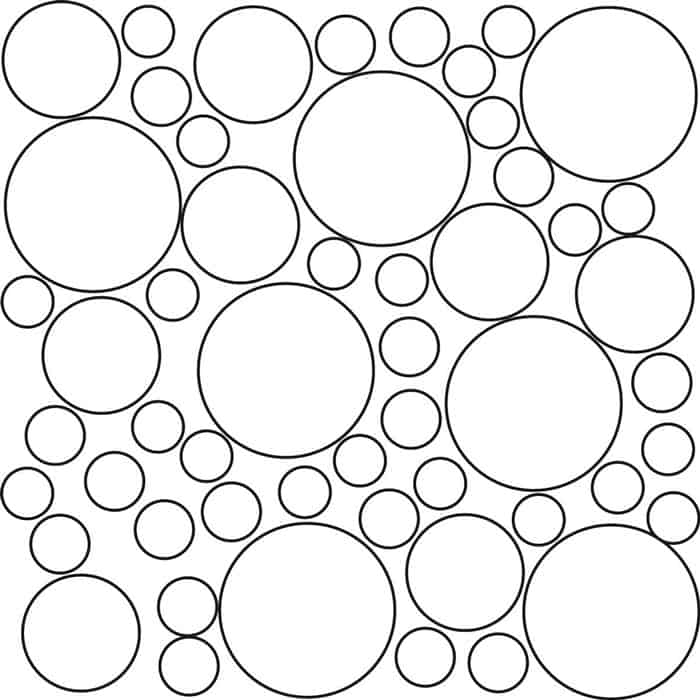
\includegraphics[width=2.5in]{images/input-circles}\label{fig:input-circles}
  }
  \hfil
  \subfloat[Circles detected within the image.]{
  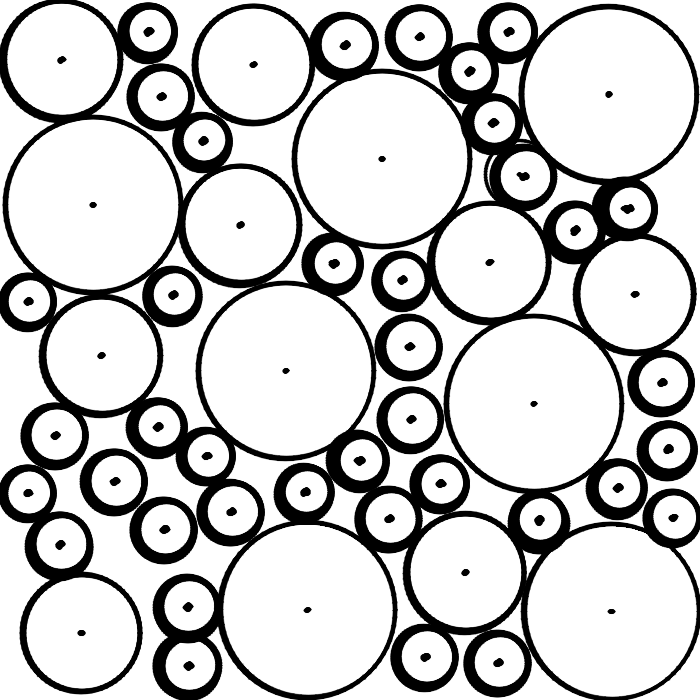
\includegraphics[width=2.5in]{images/detected-circles}\label{fig:detected-circles}
  }
  \caption{\autoref{fig:input-circles} is the input image that was used as an input to the program.\autoref{fig:detected-circles} is the output to the program when it is run.}
\end{figure*}
% As you can see in Figure \autoref{fig:detected-circles}, this is how I talk about it.






\section{Evaluation and Validation}
% Now that our
\subsection{Convolution Optimizations}



\section{Conclusion}
% 200 Words Max



\bibliographystyle{ieeetr}
\bibliography{refs}


\end{document}
